\documentclass{beamer}
\usepackage[utf8]{inputenc}

\usetheme{Boadilla}
\usecolortheme{lily}
\usepackage{amsmath,amssymb,amsfonts,amsthm}
\usepackage{mathtools}
\usepackage{txfonts}
\usepackage{tkz-euclide}
\usepackage{listings}
\usepackage{multicol}
\usepackage{adjustbox}
\usepackage{array}
\usepackage{tabularx}
\usepackage{lmodern}
\usepackage{gvv}
\usepackage{circuitikz}
\usepackage{tikz}
\usepackage{graphicx}

\setbeamertemplate{footline}
{
  \leavevmode%
  \hbox{%
  \begin{beamercolorbox}[wd=\paperwidth,ht=2.25ex,dp=1ex,right]{author in head/foot}%
    \insertframenumber{} / \inserttotalframenumber\hspace*{2ex}
  \end{beamercolorbox}}%
  \vskip0pt%
}

\usepackage{tcolorbox}
\tcbuselibrary{minted,breakable,xparse,skins}




\providecommand{\nCr}[2]{\,^{#1}C_{#2}} % nCr
\providecommand{\nPr}[2]{\,^{#1}P_{#2}} % nPr
\providecommand{\mbf}{\mathbf}
\providecommand{\pr}[1]{\ensuremath{\Pr\left(#1\right)}}
\providecommand{\qfunc}[1]{\ensuremath{Q\left(#1\right)}}
\providecommand{\sbrak}[1]{\ensuremath{{}\left[#1\right]}}
\providecommand{\lsbrak}[1]{\ensuremath{{}\left[#1\right.}}
\providecommand{\rsbrak}[1]{\ensuremath{{}\left.#1\right]}}
\providecommand{\brak}[1]{\ensuremath{\left(#1\right)}}
\providecommand{\lbrak}[1]{\ensuremath{\left(#1\right.}}
\providecommand{\rbrak}[1]{\ensuremath{\left.#1\right)}}
\providecommand{\cbrak}[1]{\ensuremath{\left\{#1\right\}}}
\providecommand{\lcbrak}[1]{\ensuremath{\left\{#1\right.}}
\providecommand{\rcbrak}[1]{\ensuremath{\left.#1\right\}}}
\theoremstyle{remark}
\newcommand{\sgn}{\mathop{\mathrm{sgn}}}
\providecommand{\abs}[1]{\left\vert#1\right\vert}
\providecommand{\res}[1]{\Res\displaylimits_{#1}}
\providecommand{\norm}[1]{\lVert#1\rVert}
\providecommand{\mtx}[1]{\mathbf{#1}}
\providecommand{\mean}[1]{E\left[ #1 \right]}
\providecommand{\fourier}{\overset{\mathcal{F}}{ \rightleftharpoons}}
%\providecommand{\hilbert}{\overset{\mathcal{H}}{ \rightleftharpoons}}
\providecommand{\system}{\overset{\mathcal{H}}{ \longleftrightarrow}}
	%\newcommand{\solution}[2]{\textbf{Solution:}{#1}}
%\newcommand{\solution}{\noindent \textbf{Solution: }}
\providecommand{\dec}[2]{\ensuremath{\overset{#1}{\underset{#2}{\gtrless}}}}
\newcommand{\myvec}[1]{\ensuremath{\begin{pmatrix}#1\end{pmatrix}}}
\let\vec\mathbf

\lstset{
%language=C,
frame=single,
breaklines=true,
columns=fullflexible
}

\numberwithin{equation}{section}

\lstset{
  language=Python,
  basicstyle=\ttfamily\small,
  keywordstyle=\color{blue},
  stringstyle=\color{orange},
  numbers=left,
  numberstyle=\tiny\color{gray},
  breaklines=true,
  showstringspaces=false
}

\title{Problem 12.765}
\author{ee25btech11023-Venkata Sai}

\date{\today}
\begin{document}

\begin{frame}
\titlepage
\end{frame}

\section*{Outline}
\begin{frame}
\tableofcontents
\end{frame}

\section{Problem}

\begin{frame}
\frametitle{Problem}
Let $\vec{v_1}=\myvec{1\\2\\0}$ and $\vec{v_2}=\myvec{2\\1\\3}$ be two vectors. The value of the coefficient $\alpha$ in the
expression $\vec{v_1} = \alpha \vec{v_2} +\vec{e}$, which minimizes the length of the error vector $\vec{e}$, is
\end{frame}
%\subsection{Literature}
\section{Solution}


\subsection{Formula}
\begin{frame}
\frametitle{Formula}
Given expression
\begin{align}
    \vec{v_1} = \alpha \vec{v_2} +\vec{e}
\end{align}
where $\vec{e}$ is the error vector\\
 For any linear system $\vec{A}\vec{x}=\vec{B}$, the least squares solution formula is given by
 \begin{align}
     \brak{\vec{A}^\top\vec{A}}\vec{x}=\vec{A}^\top\vec{B} \\
     \vec{x}= \brak{\vec{A}^\top\vec{A}}^{-1}\vec{A}^\top\vec{B}
 \end{align}
 On writing the given expression as a linear system
 \begin{align}
     \vec{v_2}\alpha =\vec{v_1}
 \end{align}
 where $\alpha$ being an 1$\times$1 vector
\end{frame}
\subsection{Conclusion}
\begin{frame}
\frametitle{Conclusion}
\begin{align}
     \vec{A}=\vec{v_2},\vec{B}=\vec{v_1}
     \end{align}
     \begin{align}
\alpha&=\brak{\vec{v_2}^\top\vec{v_2}}^{-1}\vec{v_2}^\top\vec{v_1} \\
    &= \brak{\myvec{2\\1\\3}^\top\myvec{2\\1\\3}}^{-1}\myvec{2\\1\\3}^\top\myvec{1\\2\\0} \\
     &= \brak{\myvec{2&1&3}\myvec{2\\1\\3}}^{-1}\myvec{2&1&3}\myvec{1\\2\\0} \\
     &=\brak{4+1+9}^{-1}\brak{2+2+0}\\
     &=\frac{1}{14}\brak{4}\\
     &=\frac{2}{7}
 \end{align}
 \end{frame}
 \section{Plot}
 \begin{frame}
 \frametitle{Plot}
  \begin{figure}[h!]
   \centering
   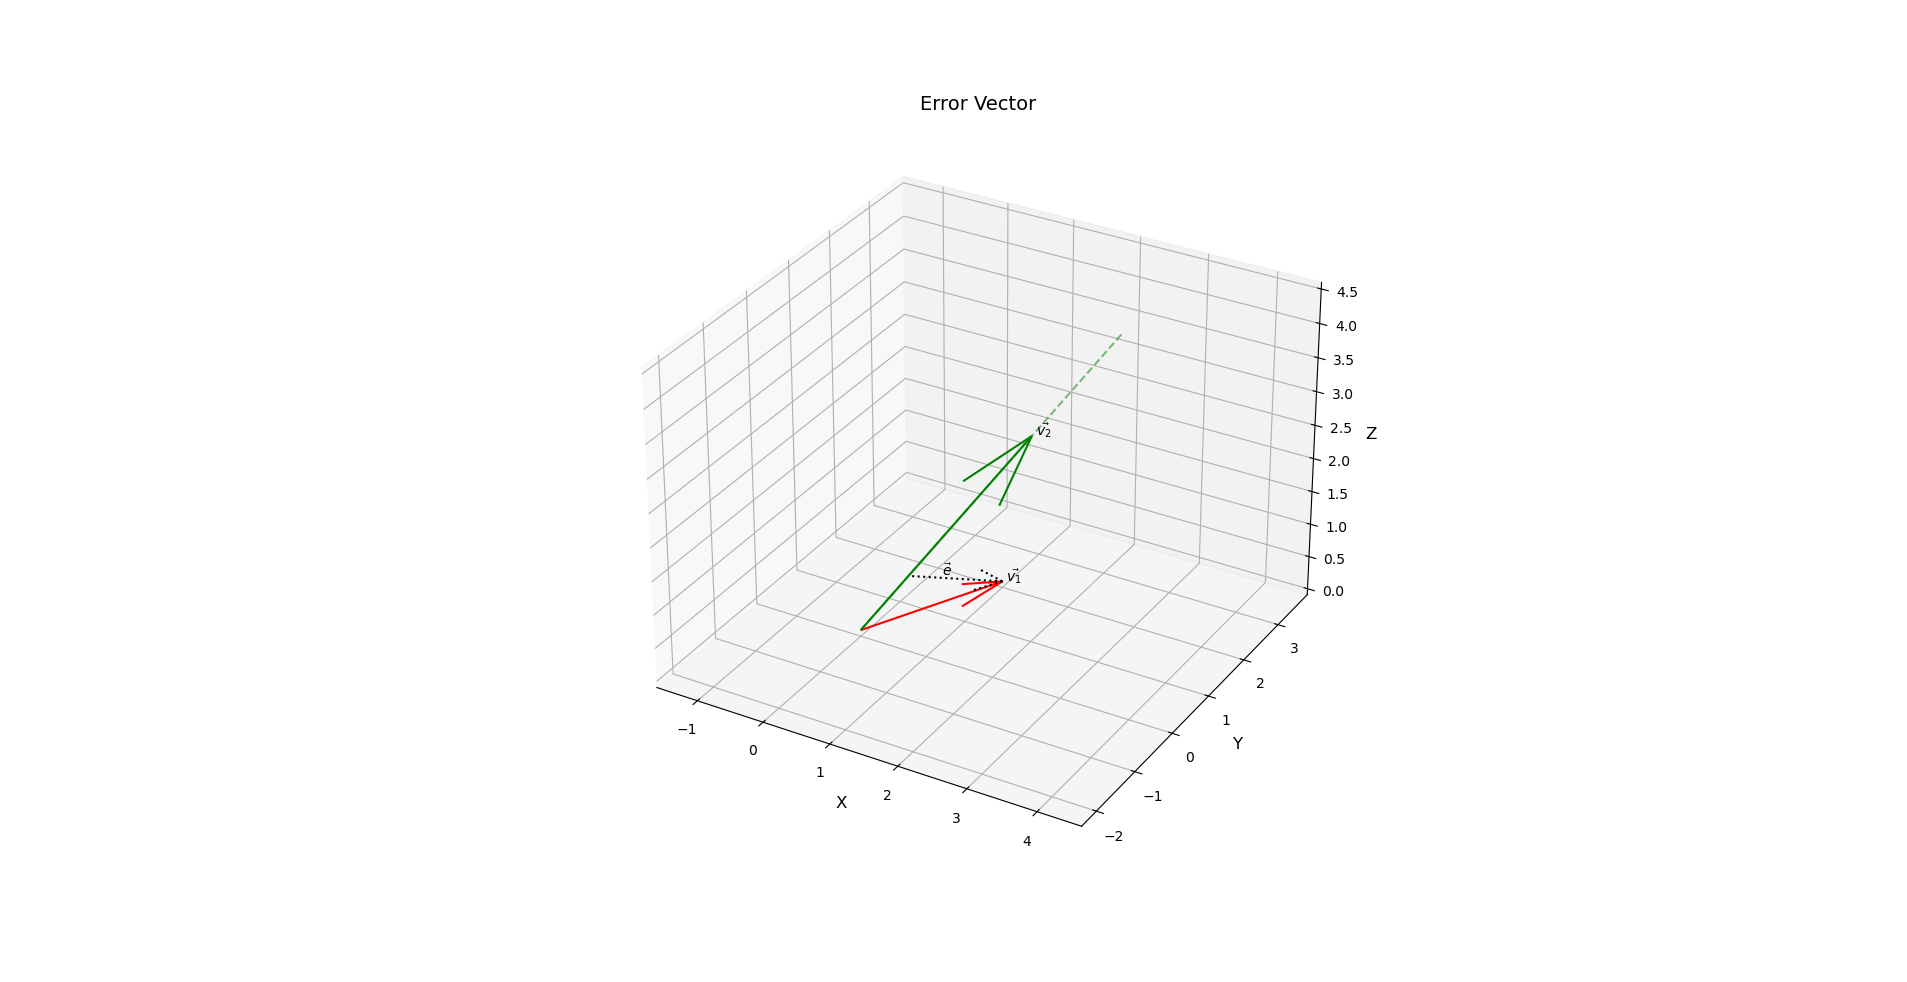
\includegraphics[width=1.\columnwidth]{figs/fig1.png}
	\caption{}
   \label{}
\end{figure}
\end{frame}
 \section{C code}
\begin{frame}[fragile]
\frametitle{C code }
\begin{lstlisting}[language=C]
void get_vectors(double* data) {
    data[0] = 1.0;
    data[1] = 2.0;
    data[2] = 0.0;
    data[3] = 2.0;
    data[4] = 1.0;
    data[5] = 3.0;
}
\end{lstlisting}
\end{frame}
\section{Python code}
 \begin{frame}[fragile]
\frametitle{Python code for calling }
\begin{lstlisting}[language=Python]
import ctypes
import numpy as np

def solve_least_squares():
    lib = ctypes.CDLL('./code.so')

    out_data = (ctypes.c_double * 6)()
    lib.get_vectors.argtypes = [ctypes.POINTER(ctypes.c_double)]
    lib.get_vectors(out_data)
    data = np.array(list(out_data))
    v1 = data[0:3]
    v2 = data[3:6]
    v2_dot_v2 = np.dot(v2, v2)
    v2_dot_v1 = np.dot(v2, v1)
    alpha = v2_dot_v1 / v2_dot_v2
    error_vec = v1 - (alpha * v2)
    return v1, v2, error_vec, alpha
\end{lstlisting}
\end{frame}
 \begin{frame}[fragile]
\frametitle{Python code for plotting }
\begin{lstlisting}[language=Python]
import matplotlib.pyplot as plt
import numpy as np
from call import solve_least_squares

v1, v2, e, alpha = solve_least_squares()

fig = plt.figure(figsize=(9, 9))
ax = fig.add_subplot(111, projection='3d')

ax.quiver(0, 0, 0, v1[0], v1[1], v1[2], color='r')
ax.text(v1[0], v1[1], v1[2], ' $\\vec{v_1}$')

line_v2 = np.array([np.zeros(3), 1.5 * v2])
ax.plot(line_v2[:, 0], line_v2[:, 1], line_v2[:, 2], 'g--', alpha=0.5)
ax.quiver(0, 0, 0, v2[0], v2[1], v2[2], color='g')
ax.text(v2[0], v2[1], v2[2], ' $\\vec{v_2}$')
projection_point = alpha * v2
\end{lstlisting}
\end{frame}
 \begin{frame}[fragile]
\frametitle{Python code for plotting }
\begin{lstlisting}[language=Python]
ax.quiver(projection_point[0], projection_point[1], projection_point[2],
          e[0], e[1], e[2],
          color='k', linestyle=':')
ax.text(projection_point[0]+0.8, projection_point[1]-0.5, projection_point[2]+0.5, '$\\vec{e}$')
ax.set_title('Error Vector',fontsize=14)
ax.set_xlabel('X',fontsize=12); ax.set_ylabel('Y',fontsize=12); ax.set_zlabel('Z',fontsize=12)
ax.legend()
ax.grid(True)
ax.axis('equal')
plt.show()

\end{lstlisting}
\end{frame}
\end{document}
